\be\label{expfn} x'{}^{i}=f^i(x^k).\ee
说 $\varphi$ 可逆，是指这些关系可以反解，
\be\label{nexpfn} x^i=k^i(x'{}^{k}).\ee
$\varphi$ 是 $Y$ 的辛同胚（而不只是微分同胚）这一条件，意味着 $\varphi^*(\omega)=\omega$，更详细地说
\be\label{nexo}\sum_{i,j}\omega_{ij}(x')\d x'{}^{i}\d x'{}^{j}=\sum_{i,j}\omega_{ij}(x)\d x^i\d x^j.\ee
当然还可以加更多条件。若 $Y$ 是复流形且 $\varphi$ 是全纯映射，则可取 $x^i$ 为局部全纯坐标，此时函数 $f^i$ 与 $k^i$ 全纯。若 $Y$ 上有一个 distinguished 的多项式函数类，则当 $f^i$ 与 $k^i$ 为多项式时，$\varphi$ 是多项式映射。

辛同胚的条件 \eqref{nexo} 有一个有趣的解释。考虑 $Y$ 的两个拷贝之积，比如 $Y\times Y'$，其中 $x^i$ 视为 $Y$ 上的坐标，$x^{i'}$ 视为 $Y'$ 上的坐标。条件 $x'{}^{i}=f^i(x^k)$，或等价地 $x^i=k^i(x'{}^{k})$，定义了中间维子流形 $L\subset Y\times Y'$。把 $Y\times Y'$ 视为带辛结构 $\omega\boxplus(-\omega)$ 的辛流形，即 $Y\times Y'$ 的辛形式是第一个因子上 $\omega$ 与第二个因子上 $-\omega$ 之和。\footnote{\label{boxes}更详细地说，若 $\pi:\h Y\to Y$ 与 $\pi':\h Y\to Y'$ 是 $\h Y=Y\times Y'$ 到两个因子的投影，$\alpha,\alpha'$ 分别是 $Y$ 与 $Y'$ 上的二形式，则定义
$\alpha\boxplus\alpha'=\pi^*(\alpha)+{\pi'}^*(\alpha')$。类似地，若 $\RR,\RR'$ 是两个因子上的线丛，则定义 $\RR\boxtimes\RR'=\pi^*(\RR)\otimes\pi'^*(\RR')$。这是 $\h Y$ 上的线丛，在第一个因子上为 $\RR$、在第二个因子上为 $\RR'$。}
式 \eqref{nexo} 意味着 $L$ 是这个实辛结构下 $Y\times Y'$ 的拉格朗日子流形。

一般地，考虑两个辛流形 $Y,Y'$ 的积 $Y\times Y'$。$Y\times Y'$ 的拉格朗日子流形 $L$ 称为 $Y$ 与 $Y'$ 之间的拉格朗日对应。若拉格朗日对应 $L$ 如上所述与 $Y,Y'$ 间的某个辛同胚相伴，则它是非常特殊的情形：若 $y_0,y_0'$ 分别是 $Y$ 与 $Y'$ 中的点，则 $L$ 与 $y_0\times Y'$ 或 $Y\times y_0'$ 的交是单点。

\begin{figure}[htbp]
 \centering
 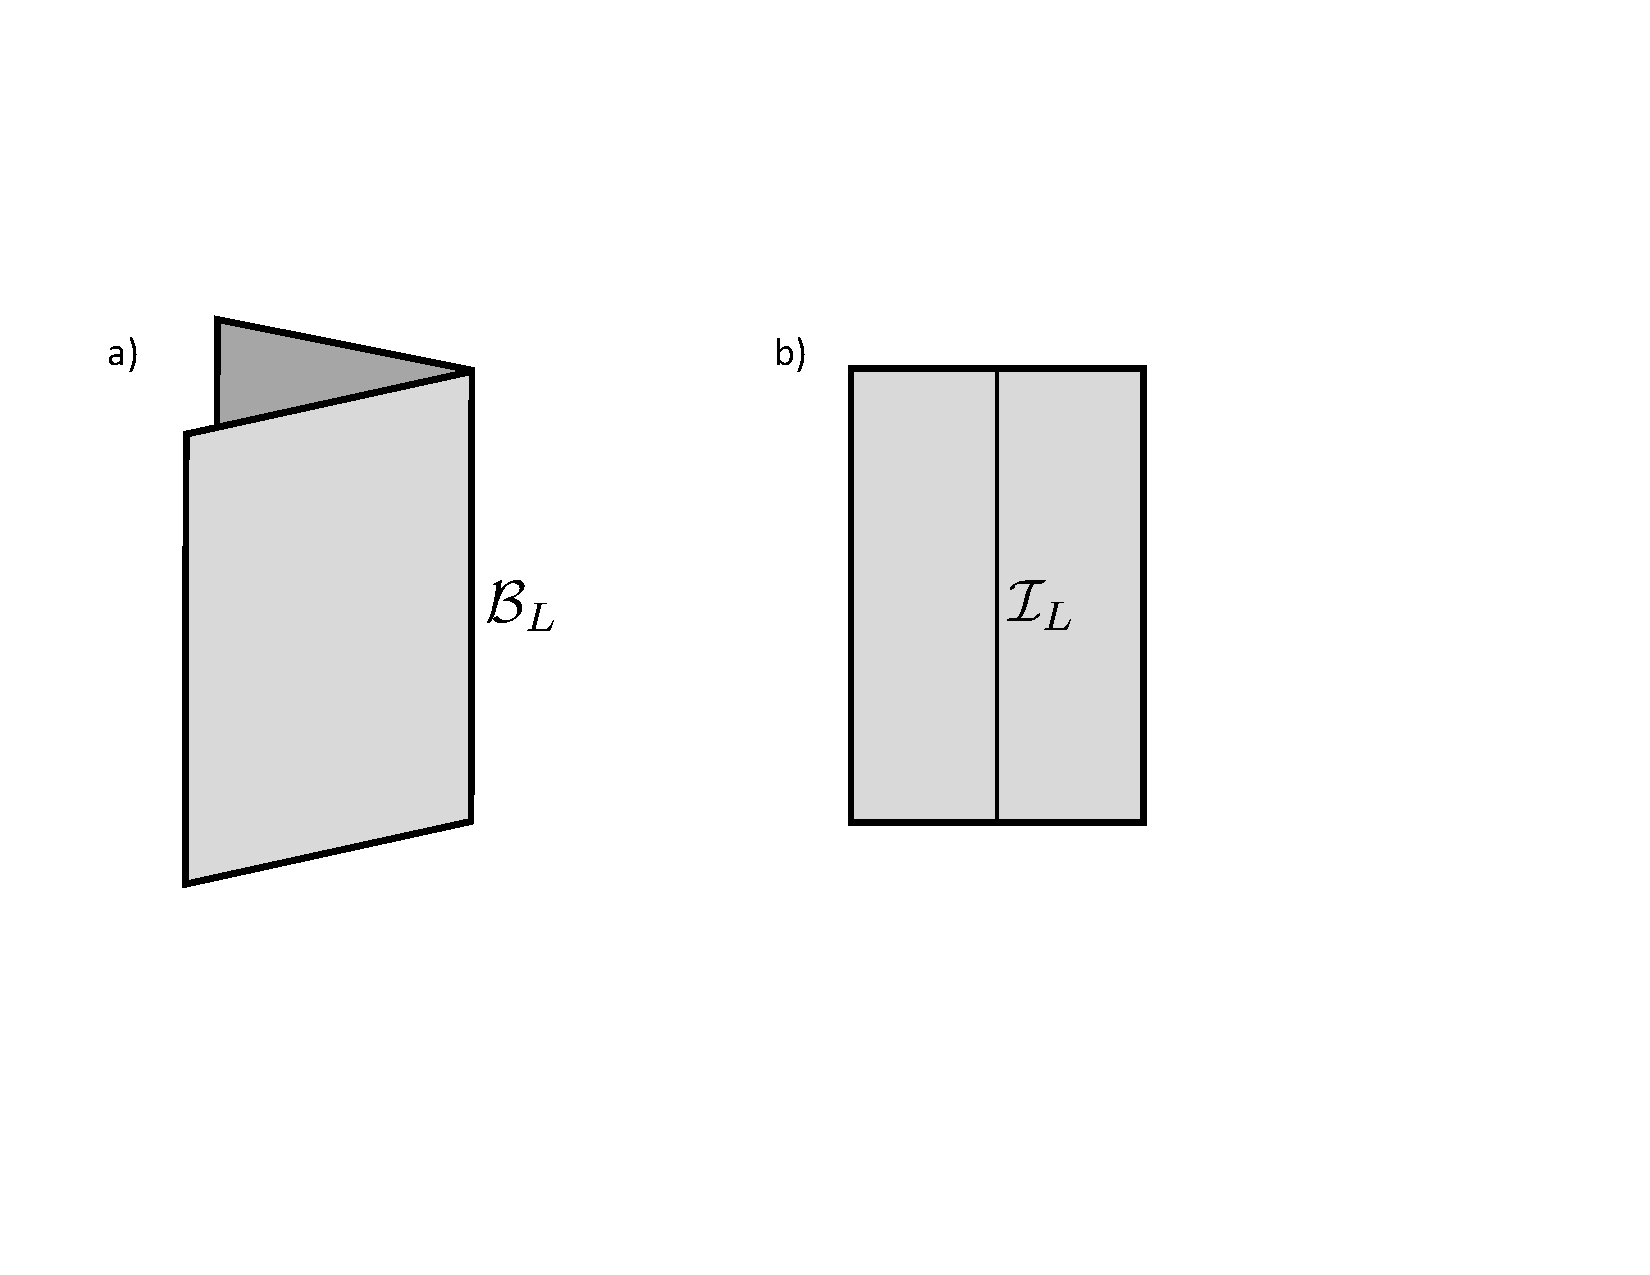
\includegraphics[width=0.72\textwidth]{figures/Folding.pdf}
 \caption{积 $Y\times Y'$ 的 $\sigma$-模型可理解为二维流形 $\Sigma$ 上的量子场，$\Sigma$ 有两张相同的叶，一张映到 $Y$、一张映到 $Y'$。(a) 我们考虑两叶仅通过一个与膜 $\B_L$ 相伴的边界条件耦合的情形。我们把这种耦合画成两叶沿边界粘合。(b) “展开”后，该膜成为靶为 $Y$（图左部）与 $Y'$（图右部）的 $\sigma$-模型之间的界面或畴壁 $\I_L$。$\I_L$ 支撑在中央竖线 $\ell$ 上。}\label{unfolding}
\end{figure}

若 $L$ 是 $Y\times Y'$ 中的拉格朗日对应，则在 $L$ 上选取平坦 $\spinc$ 结构后，可定义 $Y\times Y'$ 的 $A$-模型中的拉格朗日 $A$-膜 $\B_L$。在映射 $\Phi:\Sigma\to Y\times Y'$ 的 $\sigma$-模型中（$\Sigma$ 为二维流形），膜 $\B_L$ 的作用是沿 $\Sigma$ 边界的一部分 $\partial_0\Sigma$ 定义一个可能的边界条件。由于 $Y\times Y'$ 是简单乘积，可把 $\Sigma$ 想成有两张叶，一张映到 $Y$、一张映到 $Y'$；两叶仅沿 $\Sigma$ 的边界耦合。边界条件意味着 $\Phi$ 把 $\partial_0\Sigma$ 映到 $L\subset Y\times Y'$（边界耦合依赖于 $L$ 的 $\spinc$ 结构）。这一构造有一个有用的“展开”版本（图 \ref{unfolding}）。为此，我们沿 $\partial_0\Sigma$ 把 $\Sigma$ 的一张叶“翻过来”或展开。展开后，$\Sigma$ 被替换为二维流形 $\h\Sigma$，其中 $\partial_0\Sigma$ 不再是边界，而是内线 $\ell$。在 $\ell$ 的“左”边，$\Sigma$ 映到 $Y$；在右边，映到 $Y'$。于是在展开后的图像中，膜 $\B_L$ 被替换为 $Y$ 的 $\sigma$-模型与 $Y'$ 的 $\sigma$-模型之间的畴壁或“界面” $\I_L$。

到目前为止，这些是关于二维场论的一般论述。现在特殊化到 $Y'$ 是 $Y$ 的第二个拷贝、且我们研究的是 $Y'$ 上辛形式与 $Y$ 上辛形式反号的 $A$-模型的情形。“展开”反转 $\Sigma$ 的一张叶的定向；在 $A$-模型中，反转世界面定向等价于反转辛形式的符号。由于我们从两个 $Y$ 拷贝上相反的辛结构出发，展开后辛结构处处相同，我们就简单地得到单个 $Y$ 拷贝的普通 $A$-模型。先前图像中 $Y\times Y'$ 的 $A$-模型里的 $A$-膜 $\B_L$，展开后变成 $Y$ 的 $A$-模型中的拓扑畴壁或界面 $\I_L$。称此界面为“拓扑的”，意思是它可以在 $\Sigma$ 中自由移动而不影响 $A$-模型的可观测量。\footnote{特别地，可以把拓扑界面上移到边界，在那里它与已有边界条件结合成新的边界条件。这定义了数学语言中可称为边界条件范畴上的函子的东西。这在某些应用（包括几何 Langlands）中很重要；但这里我们将用拓扑界面定义普通的量子算符。}

\begin{figure}[htbp]
 \centering
 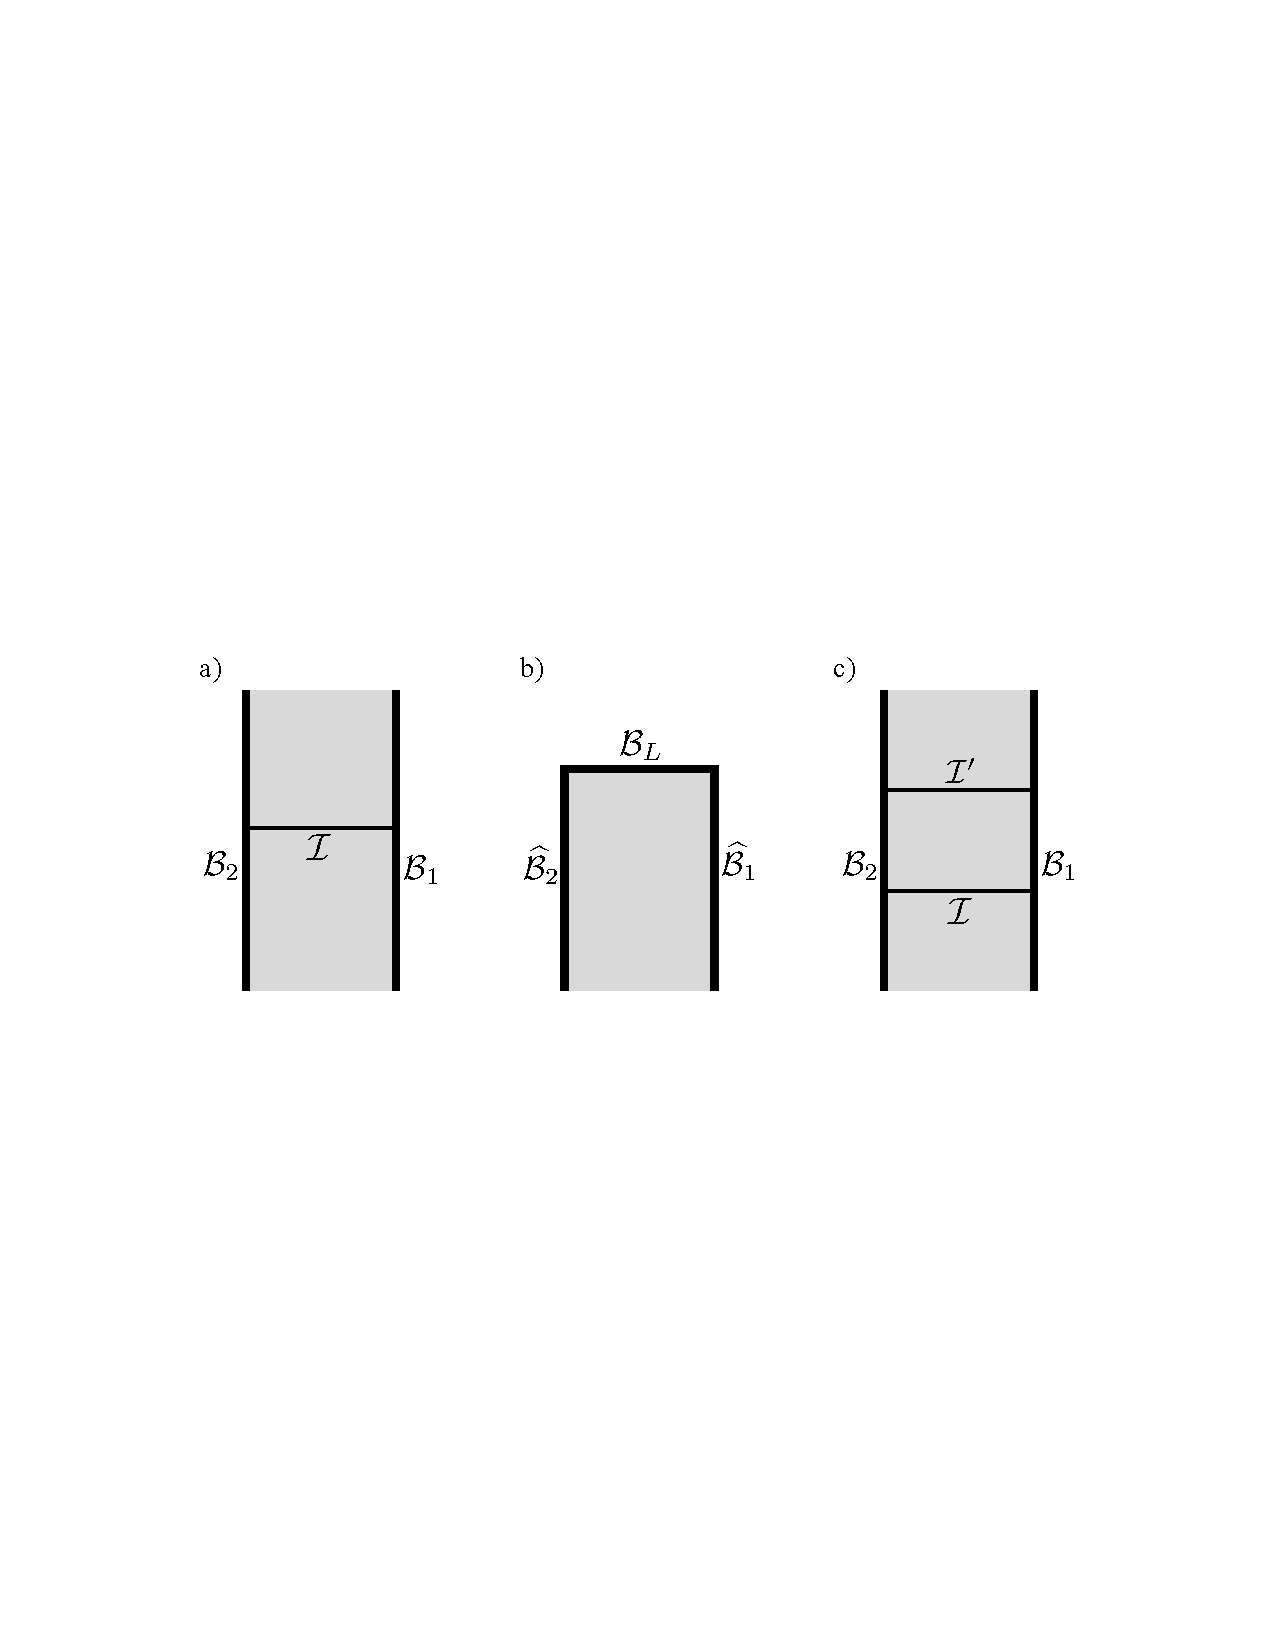
\includegraphics[width=0.9\textwidth]{figures/correspondence.pdf}
 \caption{(a) 用于定义作用在 $A$-模型物理态空间 $\Hom(\B_1,\B_2)$ 上的算符的拓扑界面 $\I$。左右两侧是膜 $\B_1$ 与 $\B_2$；水平线代表界面 $\I$。在图中水平线与边界相遇的“端点”处必须提供额外信息。一个物理态从条带底部进入，与界面相互作用，再从顶部出来。若从上往下读图，它描述 $\Hom(\B_2,\B_1)$ 上的对偶或转置算符。(b) 此图由 (a) 沿支撑界面 $\I_L$ 的曲线 $\ell$ “折叠”得到。折叠把 $\ell$ 换成现在由膜 $\B_L$ 标记的边界。左右两侧，$\h\B_1$ 与 $\h\B_2$ 是膜 $\B_1$ 与 $\B_2$ 的折叠或加倍版本。正文的叙述从这一折叠图像开始，然后展开得到前一图像。(c) 算符的合成来自相伴拓扑界面 $\I$ 与 $\I'$ 连同相应端点的合成。在拓扑场论中，可以融合两个界面，并利用局部算符的算符乘积展开的类比来合并它们的端点。}\label{correspondence}
\end{figure}

拓扑界面或畴壁可用于定义作用在 $A$-模型物理态空间上的算符。基本想法如图 \ref{correspondence}(a) 所示。条带 $\R\times I$（$I$ 为单位区间）上、边界条件与膜 $\B_1,\B_2$ 相伴的 $A$-模型描述 $\Hom(\B_1,\B_2)$。现在加入一个水平横穿条带的拓扑界面 $\I$。必须提供一些信息来说明界面与条带左右边界相遇处发生什么。假设这已以满意的方式完成，则条带上的路径积分定义一个作用在 $\Hom(\B_1,\B_2)$ 上的算符 $\O$。从下往上读图，$\Hom(\B_1,\B_2)$ 中的一个态从底部进入并与界面相互作用；然后一个可能不同的 $\Hom(\B_1,\B_2)$ 中的态从顶部出来。（从上往下读，同一图像描述对偶向量空间 $\Hom(\B_2,\B_1)$ 上的对偶或转置算符。）

我们把 $\I$ 在条带左边界或右边界上的终点称为 $\I$ 与 $\B_1$ 或 $\B_2$ 的“端点”。要理解界面的端点，其实方便的是回到折叠图像。我们沿界面折叠图 \ref{correspondence}(a) 的世界面，使界面的轨迹成为边界（正如它在图 \ref{unfolding}(a) 中原本那样）。在折叠图像（图 \ref{correspondence}(b) 所示）中，界面 $\I$ 来自 $Y\times Y'$ 的 $A$-模型中的膜 $\B_L$；同样，左右边界由膜 $\h\B_1$ 与 $\h\B_2$（$\B_1$ 与 $\B_2$ 的折叠版本）标记。$\I$ 在 $\B_1$ 或 $\B_2$ 上的端点，正是第 \ref{ccb} 节与图 \ref{strip} 所研究的 $(\B_L,\h\B_1)$ 或 $(\h\B_2,\B_L)$ 角。换言之，这些角是 $\Hom(\B_L,\h\B_1)$ 与 $\Hom(\h\B_2,\B_L)$ 的元素。它们正是我们在第 \ref{comparing} 节与附录 \ref{details} 中详细讨论过的那类东西。

一旦选定了角，拉格朗日对应就定义作用在 $A$-模型物理态上的算符。特别地，拉格朗日对应可用于定义实辛子流形 $M\subset Y$ 的膜量子化中的算符。正如第 \ref{ques} 节所指出的，若 $Y$ 使得全纯函数代数 $\A_0$ 相对“小”、小到不足以有效刻画 $M$ 的量子化，这一点就尤其重要。由对应导出的算符在这种情形中很重要。
